% Created 2022-01-25 wto 11:20
% Intended LaTeX compiler: pdflatex
\documentclass[11pt]{article}
\usepackage[utf8]{inputenc}
\usepackage[T1]{fontenc}
\usepackage{graphicx}
\usepackage{grffile}
\usepackage{longtable}
\usepackage{wrapfig}
\usepackage{rotating}
\usepackage[normalem]{ulem}
\usepackage{amsmath}
\usepackage{textcomp}
\usepackage{amssymb}
\usepackage{capt-of}
\usepackage{hyperref}
\usepackage{minted}
\usepackage[pl, polish]{babel}
\usepackage[margin=1in]{geometry}
\author{Patryk Kaniewski}
\date{\today}
\title{Sprawozdanie \\
Badanie róznych algorytmów szyfrowania - szyfrowanie asymetryczne}
\hypersetup{
 pdfauthor={Patryk Kaniewski},
 pdftitle={Sprawozdanie \\
Badanie róznych algorytmów szyfrowania - szyfrowanie asymetryczne},
 pdfkeywords={},
 pdfsubject={},
 pdfcreator={Emacs 27.2 (Org mode 9.4.4)}, 
 pdflang={Polish}}
\begin{document}

\maketitle
\tableofcontents \clearpage

\section{Cryptool}
\label{sec:org30aa986}
Cryptool jest narzędziem do badania róznych algorytmów szyfrowania i funkcji skrótu (\emph{hash function}). Jest to narzędzie głownie edukacyjne chociaż można go używać do szyfrowania zwykłych wiadomości np. z pliku tekstowego

\subsection{Wspierane algorytmy symetryczne}
\label{sec:org8e3c720}
Jcrypttool wspiera wiele symetrycznych algorytmów szyfrowania, oferuje również poza szyframi rożnymi algorytmami szyfrowania symetrycznego, funkcje hashujące oraz kryptografie klucza publicznego. Jest to narzędzie open source, stworzone w jezyku Java i dzięki temu jest dostępne na wszystkich platformach z JVM. Można też w nim znaleźć historyczne metody do zachowania poufności takie jak szyfr cezara czy XOR.


\subsection{Wybrane przypadki}
\label{sec:orgec8fab8}
Całe ćwiczenie zostało wykonane za pomocą narzędzi lini polecenia na systemie Linux.

Przygotowane zostały dwa pliki z tekstem (50 bajtowy plik i 100 bajtowy plik) zakodowanym w domyślnym utf-8.

\subsubsection{50 bajtowy plik}
\label{sec:org2c115eb}
Plik 50 bajtowy jest przygotowany w dwóch wersjach, używając małych i dużych liter aby sprawdzić jak wpływa to na funkcje hashujące tekst.
\begin{minted}[]{sh}
cat examples/50bfile.txt
hexdump examples/50bfile.txt
awk '{print toupper($0)}' < examples/50bfile.txt > examples/50bupper.txt
cat examples/50bupper.txt
hexdump examples/50bupper.txt
\end{minted}

\begin{verbatim}
Real sold my in call. Invitation on an advantages

0000000 6552 6c61 7320 6c6f 2064 796d 6920 206e
0000010 6163 6c6c 202e 6e49 6976 6174 6974 6e6f
0000020 6f20 206e 6e61 6120 7664 6e61 6174 6567
0000030 0a73                                   
0000032
REAL SOLD MY IN CALL. INVITATION ON AN ADVANTAGESy

0000000 4552 4c41 5320 4c4f 2044 594d 4920 204e
0000010 4143 4c4c 202e 4e49 4956 4154 4954 4e4f
0000020 4f20 204e 4e41 4120 5644 4e41 4154 4547
0000030 0a53                                   
0000032
\end{verbatim}
Jak widać tekst zakodowany w UTF-8 różni się pomiedzy dużymi i małymi literami nieznacznie. Każdy bajt przesunięty jest o 0x20 (poza kropką i dużą litera na początku zdania).

\subsubsection{100 bajtowy plik}
\label{sec:org12a1eae}

Plik 100 bajtowy jest przygotowany z części tekstu \emph{lorem ipsum}
\begin{minted}[]{sh}
cat examples/100bfile.txt
hexdump examples/100bfile.txt
\end{minted}

\begin{verbatim}
Impedit dolorem quo ullam quam et et a.
Ea quo laborum eaque sint hic. Laborum ea et in nesciunt cu

0000000 6d49 6570 6964 2074 6f64 6f6c 6572 206d
0000010 7571 206f 6c75 616c 206d 7571 6d61 6520
0000020 2074 7465 6120 202e 6145 7120 6f75 6c20
0000030 6261 726f 6d75 6520 7161 6575 7320 6e69
0000040 2074 6968 2e63 4c20 6261 726f 6d75 6520
0000050 2061 7465 6920 206e 656e 6373 7569 746e
0000060 6320 0a75                              
0000064
\end{verbatim}

\section{Funkcje Skrótu}
\label{sec:orgacf147e}
Funkcja skrótu (funkcja haszująca, \emph{hash function}) jest funkcja której wynikiem jest stałej długości ciąg bitów niezależny dla dowolnego argumentu funkcji. Sa wykorzystywane w kryptografi głownie w połączeniu z \emph{saltowaniem} - dodawaniem losowego ciągu znaków do hasła w celu uniemożliwienia ataków typu \emph{rainbow table} (prekalkukowane hashe haseł - wymagane wtedy jest tylko porownanie hashów z wykradniętej bazy danych z \emph{rainbow table}, czyli tabelą prekalkulowanych hashy).

Funkcje haszujące sa również wykorzystywane w porownywaniu plików, jest to szybsze od porównywania bitowego jak i również może byc dystrybuowane pomiedzy róznymi systemami (zwykle wynik funkcji hashującej jest udostępniany z plikiem online aby sprawdzić poprawność pobierania  oraz oryginalność danego pliku).

Funkcje hashowe które zostały złamane (np. kolizje lub złozoność liczbowa) nadal mogą być wykorzystywane do porównywania plików jednak tylko przed losowymi zmianami i nie jest to bezpieczne dla żadnych innych rozwiązań. W obecnych czasach wypierania jest funkcja SHA1 oraz MD5.

\subsection{SHA2 (SHA256)}
\label{sec:org23ee42c}
\begin{minted}[]{sh}
sha256sum examples/50bfile.txt examples/50bupper.txt  examples/100bfile.txt
\end{minted}

\begin{verbatim}
1174aa85039138644566c6c8776bf939682b17fab4ec1bdef8860180b164123d  examples/50bfile.txt
594e9404692b199dc6f1ec6fb81679e383e022b7c19e0e05cfc0f76bdf86adfd  examples/50bupper.txt
246b9020507c302460536cc2f9383b1ac3646e01ae86e35f0b851a2303a395d0  examples/100bfile.txt
\end{verbatim}


SHA256 zgodnie ze swoją nazwą podaje wynik długości 256 bitów za pomocą algorytmu SHA2.

\subsection{SHA2 (SHA512)}
\label{sec:org8b8fd82}
\begin{minted}[]{sh}
sha512sum examples/50bfile.txt examples/50bupper.txt  examples/100bfile.txt
\end{minted}

\begin{verbatim}
: 0f5acbc8ef589654b412ff4306e30c14da7325037e3e12bb8b996623deb8f741
: a4313c2f5bbd6f3292835c1f713f1a2ec23ab289edcc7184d764529abf168646  examples/50bfile.txt
: 3cd96f4ede8f596af82e6f6b87af5190adb945138614d3082ccaa66801924344
: de3c2e63ff3423c8026b324e27745bcf8c4fd03b74f21fac0580fb4295524610  examples/50bupper.txt
: 141b856ad7a435b3b14b6f89b2aee4e742aa95d8d1fa6bc44e348e7cd38911af
: 585b409bab34d18842bd282c14261d08a56aac05e8236432081f3c999e156677  examples/100bfile.txt
\end{verbatim}
SHA512 zgodnie ze swoją nazwą podaje wynik długości 512 bitów za pomocą algorytmu SHA2.
\subsection{MD5}
\label{sec:orge4f6ec9}
\begin{minted}[]{sh}
md5sum examples/50bfile.txt examples/50bupper.txt examples/100bfile.txt
\end{minted}

\begin{verbatim}
929e763b742a5f79cf50010ffa4c8d2a  examples/50bfile.txt
0bd8394efa522406e9636ab69a05d1fe  examples/50bupper.txt
1014b1df517ab1f8827a0c30549c7a9b  examples/100bfile.txt
\end{verbatim}


Funkcja MD5 podaje wynik w postaci 128bitowej liczby.
\subsection{RIPEMD-160}
\label{sec:org43fae25}
\begin{minted}[]{sh}
rhash --ripemd160 examples/50bfile.txt examples/50bupper.txt  examples/100bfile.txt
\end{minted}

\begin{verbatim}
64c6222a3ec147465aa108fdf855fdafb3e92f8c  examples/50bfile.txt
a4e8a21c1ac8946cfd9090e706694dfa88a4499f  examples/50bupper.txt
99e87f6bc237fd1925ff0d85e9c8e6244dd6ea48  examples/100bfile.txt
\end{verbatim}


Funkcja RIPEMD-160 zgodnie z nazwa posiada wynik 160 bitowy.
\section{Podpis Cyfrowy}
\label{sec:org10348b2}
\subsection{PGP}
\label{sec:org831d7e7}
openPGP (\emph{Pretty Good Privacy} z ang. \emph{Dosyć dobra prywatność}), jest standardem szyfrowania i podpisywania cyfrowego dokumentów (RFC2440->RFC4880), stworzonego na potrzeby bezpiecznej komunikacji za pomocą niezabezpieczonego systemu email.

W celu zapewnienia uwierzytelnienia (Podpisu cyfrowego) PGP używa funkcji hashującej oraz infrastruktury klucza publicznego.

\begin{enumerate}
\item Nadający tworzy wiadomość
\item Oprogramowanie generuje hash wiadmości
\item Oprogramowanie generuje podpis z hashu wiadomości oraz klucza prywatnego nadającego
\item Podpis jest załączany do wiadomości
\item Oprogramowanie odbiorcy generuje hash wiadomości
\item Oprogramowanie odbiorcy porównuje podpis z otrzymaną wiadomościa.
\end{enumerate}

\subsubsection{Używanie PGP (gnuPGP)}
\label{sec:orgb4feb77}
\begin{minted}[]{sh}
rm examples/50bfile.sig
gpg --output examples/50bfile.sig --sign examples/50bfile.txt
hexdump examples/50bfile.sig
\end{minted}

\begin{verbatim}
0000000 01a3 0a01 f502 90fd 030d 0800 a301 abef
0000010 84ec a4fd 019f 43ac 0b62 3035 6662 6c69
0000020 2e65 7874 6174 ceef 52ea 6165 206c 6f73
0000030 646c 6d20 2079 6e69 6320 6c61 2e6c 4920
0000040 766e 7469 7461 6f69 206e 6e6f 6120 206e
0000050 6461 6176 746e 6761 7365 890a b301 0004
0000060 0801 1d00 2116 4504 e0ac da1c c41a ba32
0000070 708c a338 abef 84ec a4fd 059f 6102 ceef
0000080 00ea 090a a310 abef 84ec a4fd 2f9f 0bb9
0000090 7dff 9d2e 32b0 650d 50c8 277d 9bf0 7a00
00000a0 1f93 0b2a 3c16 e968 178a 5b70 9173 aab8
00000b0 e356 a9a9 5de3 a088 223b 39a2 88c0 a7a1
00000c0 74f1 1ccd 9261 4ee5 67bf b87a 8187 5e95
00000d0 a715 0dff 7e6f c67d f90f f42a e6dc d30c
00000e0 7602 9407 6d4e 824e 97b7 de5d 8afb fa68
00000f0 cc54 e5ee 2099 6927 1fc5 7eca 8845 2fc4
0000100 176b 166b a28c 326c 669d fb89 6945 d556
0000110 8b81 e435 1d95 2459 7697 d1d4 eebf e42e
0000120 d86b 7e5f 40e6 b772 d9b1 3e9f 0fda da0f
0000130 4153 de84 ea91 0bde 0524 6ebf 093c b3fb
0000140 4d7b 6986 622b 68eb a1b3 8750 ce6b e72a
0000150 e362 3c87 eaee dd3a f2aa 615f 2c11 7ac4
0000160 8606 0319 fda4 594c 3b98 6c72 9a49 733f
0000170 9b95 f9e0 597c 5ed0 fb36 0f4a ce32 8ffa
0000180 947f d2a5 cb33 0e5a 681c fedf 1a62 35b2
0000190 4504 ef8b 3021 ee7f d8a7 c1e2 d002 22ee
00001a0 09bb 00bd da9b 045c 996c 7ba7 d14f e79d
00001b0 9b51 af47 e92c eca6 ba3e 295e 2b98 66fe
00001c0 e634 d53b 072f f7ef 0ace 4bf7 cd75 a069
00001d0 5f04 e46c 3cd4 8896 5f2f 9edd 3781 74fb
00001e0 f430 9a37 399d a53b 6396 6e7e b923 67ba
00001f0 ed88 ca2b aee1 58a0 9ace 4292 d5e7 a50d
0000200 91d9 836e 2d40 246d 61c3 2ed1 54f8 57ff
0000210 00a9                                   
0000211
\end{verbatim}

Pierwsza część (0x8d bajtów) podpisanej wiadomości jest taka sama, pozostała cześć zmienia się za każdym razem gdy wiadomość jest podpisywana. Na początku jest nagłowek z informacjami o podmiocie który podpisał dokument, jakie algorytmy zostały wykorzystane w podpisie oraz oryginalna nazwa dokumentu oraz \emph{plaintext} wiadomości lub skompresowana wiadomość, po naglówku jest dołączany podpis cyfrowy.
\begin{figure}[htbp]
\centering
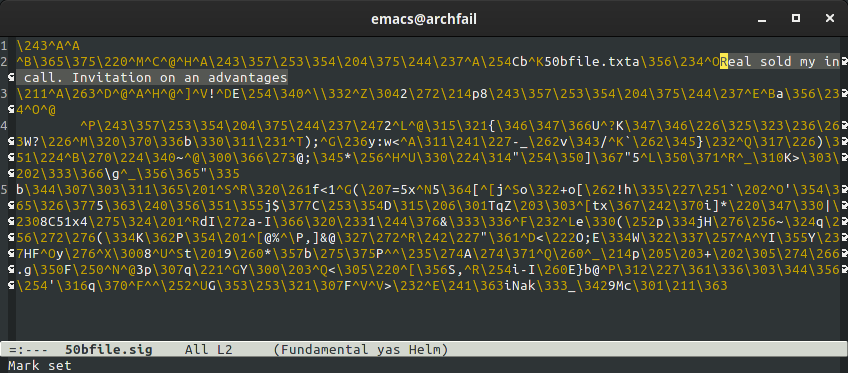
\includegraphics[width=.9\linewidth]{./data/plaintext.png}
\caption{Widoczny tekst w podpisanej wiadomości}
\end{figure}

\begin{figure}[htbp]
\centering
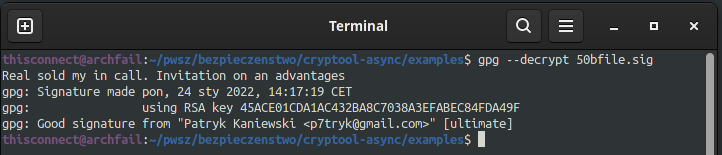
\includegraphics[width=.9\linewidth]{./data/podpis.png}
\caption{Potwierdzenie autentyczności wiadomości}
\end{figure}

\begin{verbatim}
Real sold my in call. Invitation on an advantages
\end{verbatim}


Po podpisaniu pliku możemy go zamienić w naszą wiadomość za pomocą \texttt{-{}-decrypt}

\begin{minted}[]{sh}
gpg --output examples/50bfile.dec.txt --decrypt examples/50bfile.sig
diff examples/50bfile.dec.txt examples/50bfile.txt -s
\end{minted}

\begin{verbatim}
Files examples/50bfile.dec.txt and examples/50bfile.txt are identical
\end{verbatim}


Możemy zobaczyć ró
\section{Podsumowanie}
\label{sec:org897e6af}

Szyfrowanie asymetryczne jest wykorzystywane obecnie na codzień przez miliardy ludzi, czy to używając hybrydowego podejscia do generowania kluczy sesji w HTTPS/TLS, poprzez pobieranie plików z sieci aż do podpisywania cyfrowego dokumentów i innych tworów (np. oprogramowania). Kryptografia klucza publicznego oraz metody wymiany ich kluczy pozwalają naszej przeglądarce zaufać stronie bankowości internetowej i wyswietlić zieloną kłódkę. Niestety nadal kryptografia polega głównie na wymienieniu kluczy za pomocą innych metod niż online. Patrząc przez przypadki takie jak Lenovo \emph{superfish} nadal polega na zaufaniu bazie certyfikatów dostarczonej poprzez przeglądarkę, system operacyjny, sprzęt komputerowy oraz na wydaniu poprawnych certyfikatów przez urzędy certifikacji zarówno lokalne, jak i krajowe a także największych graczy jak Google.
\end{document}
